% !TEX encoding = UTF-8 Unicode
\documentclass[10pt, conference, letterpaper]{IEEEtran}
\IEEEoverridecommandlockouts
% The preceding line is only needed to identify funding in the first footnote. If that is unneeded, please comment it out.
\usepackage{cite}
\usepackage{amsmath,amssymb,amsfonts}
\usepackage{algorithmic}
\usepackage{lipsum}  
\usepackage{graphicx}  
\usepackage{pdfpages}
\ifCLASSOPTIONcompsoc  
\usepackage[caption=false, font=normalsize, labelfont=sf, textfont=sf]{subfig}  
\else  
\usepackage[caption=false, font=footnotesize]{subfig}  
\fi  
\usepackage{textcomp}
\usepackage{xcolor}
\usepackage[ruled,linesnumbered,lined,boxed,commentsnumbered]{algorithm2e}

\usepackage{multirow}
\def\BibTeX{{\rm B\kern-.05em{\sc i\kern-.025em b}\kern-.08em
    T\kern-.1667em\lower.7ex\hbox{E}\kern-.125emX}}
\begin{document}

\title{A NFV Acceleration Scheme Based on Programmable Data Plane\\
}

%\author{\IEEEauthorblockN{1\textsuperscript{st} Hanyu ZHAO}
%\IEEEauthorblockA{\textit{dept. name of organization (of Aff.)} \\
%\textit{name of organization (of Aff.)}\\
%City, Country \\
%email address or ORCID}
%\and
%\IEEEauthorblockN{2\textsuperscript{nd} Qing LI}
%\IEEEauthorblockA{\textit{dept. name of organization (of Aff.)} \\
%\textit{name of organization (of Aff.)}\\
%City, Country \\
%email address or ORCID}
%\and
%\IEEEauthorblockN{3\textsuperscript{rd} Yong JIANG}
%\IEEEauthorblockA{\textit{dept. name of organization (of Aff.)} \\
%\textit{name of organization (of Aff.)}\\
%City, Country \\
%email address or ORCID}
%}

\maketitle


\begin{abstract}
To be written
~\\\\\\\\\\\\\\\\\\\\\\\\\\\\\\\\\
\end{abstract}

\begin{IEEEkeywords}
NFV, Programmable Data Plane, SFC
\end{IEEEkeywords}

\section{Introduction}
Network Functions (NFs) such as load balancers, firewalls, intrusion detection systems, etc. are traditionally deployed on proprietary devices called middleboxes to provide specific services for traffic. A flow typically requires to traverse serveral NFs in order to form Service Function Chain (SFC).  These massive proprietary physical devices have brought in the problem of network rigidity and difficulty in network management and infrastructure expansion.

Network Function Virtualization (NFV) was introduced as a new network paradigm to address the limitations of dedicated middleboxes. NFV offers great flexibility and scalability of service provision with lower cost by decoupling network functions from the underlying specialized hardware and realizing them on common Commercial-Off-The-Shelf (COTS) devices.
Nevertheless, the benefits of NFV comes with performance compromises. The giant performance gap between general-purpose devices and dedicated middleboxes could result in considerable latency costs. 
One VNF could add about 600 microseconds of delay to packets in addition to the overhead from transmitting packets from NIC to CPU through PCIe.
Meanwhile, more CPU cores are needed to deploy VNFs, resulting in fewer resources for service provision\cite{Pontarelli2019}.

Recently, some research efforts have been devoted to accelerate NFV, which could be divided into two types. 
1) NF Architecture Optimization. For example, OpenBox proposes NF modularization and improves overall performance by sharing common building blocks between NFs. Moreover, NFP innovatively adopts NF parallelism to improve NFV performance. 
2) Packet I/O Acceleration. Some works (NetBricks, DPDK, ClickOS, NetVM, Netmap) propose to achieve NF acceleration by optimizing packet delivery from NIC to VM, or between the VMs.
However, software-based solutions still cannot bridge the giant gap in performance.

With the advent of Programmable Data Planes (PDP), using data planes to offload NFs is gradually seen as an effective method to improve NFV performance. 
In Software Defined Networking (SDN) context, the control plane is the centralized control element in charge of making routing and traffic engineering decisions and managing data plane devices. The data plane, in contrast, is responsible solely for executing the packet processing policy set by the control plane. The data plane will perform packet processing policy set by controller through southbound API, and can be rapidly and systematically reconfigured thus providing programmablity\cite{bifulco2018survey}. The data plane functionality may be implemented in many platforms including ASIC, FPGA and netwrk processor.

Programmable data plane has processing capabilities that match line rate (e.g., 12.8 Tbps of Barefoot Tofino ASIC), and can flexibly implement complex network functions through programming packet processing logic. For example, by installing and managing IP mapping rules of flows, Network Address Translation (NAT) could be implemented on programmable switches. In addition, offloading NF in the data plane helps reduce the influence of traffic routing loop problem in NFV network, and can effectively reduce the usage of CPU cores to ensure the provision of service.

Due to the features of PDP, there are two critical challenges of NF offloading: 
1) Service Chaining. Different flows in network have diverse and dynamic SFC requirements. NFs in PDP should be organized to support multiple service chains and provide flexible reconfigurability for operators to cope with changing needs. To address this issue, a naive method is to implement one service chain in one programmable switch, which clearly lacks scalability and is not able to cope with ever-changing requirements[]. Hyper4 takes another way to fully realize virtualization by configure match filed and instructions at runtime at the cost of massive memory usage[].
2) Stateful Operations. Operation on states is widely involved in NF behaviors (e.g., a big flow detector would access its counter to decide whether to alert the controller). 

\textbf{to select from two versions}

In order to reduce the switch-to-controller's signaling overhead of state access and transition, the stateful function logic should be entirely offloaded to switch. Moreover, state consistency, i.e., packets belonging to the same flow processing the same state, should be strictly ensured.

However, current PDP platforms lack focus on paradigm of high-level stateful applications. For example, OpenFlow provides little support for maintaining states in switch where flows are not able to react differently when state changes. In contrast, FPGA offers great program flexibility, but is not operator-friendly with hardware description language.


To conquer the above challenges, we design STH, a flexible and high-performance NF management framework which leverages PDP to offload NFs. STH can allocate Hardware-based NFs (HNF) to dynamic traffic to minimize the impact on data plane. 
We adopted P4 (Programming Protocol-independent Packet Processors) switch as the data plane to offload NFs and designed a P4-based NF implementation abstraction composed of pipeline tables considering both stateless and stateful NFs, where state access and transition operations are entirely inside the switch. To effectively react to dynamic traffic with diverse SFC requirements, we designed the two-stages NF mapping algorithm including static path generation algorithm and dynamic path selection algorithm in the control plane. Our implementation on (name of hardware switch) switch shows that PDP is feasible to offload NF and achieves high performance with line rate.


%(1) Proposed NFV management platform based on P4 platform, including NF abstraction, NF initialization, service chaining and NF runtime management. System supports the realization of both stateful and stateless NF.
%
%(2) Designed the two-step NF mapping algorithm in the system control plane decision layer, which automatically selects the optimal NF placement for the incoming traffic and improves system performance while minimizing the impact on the data plane in the hybrid NF environment.
%
%(3) Provided simple NF management interface. Through the system's translation layer, the NF management commands are automatically translated into flow table rules in the corresponding switch, which could efficiently reduce the workload of the operator.
%
%(4) Hardware deployment.



\begin{figure}[t]
\centerline{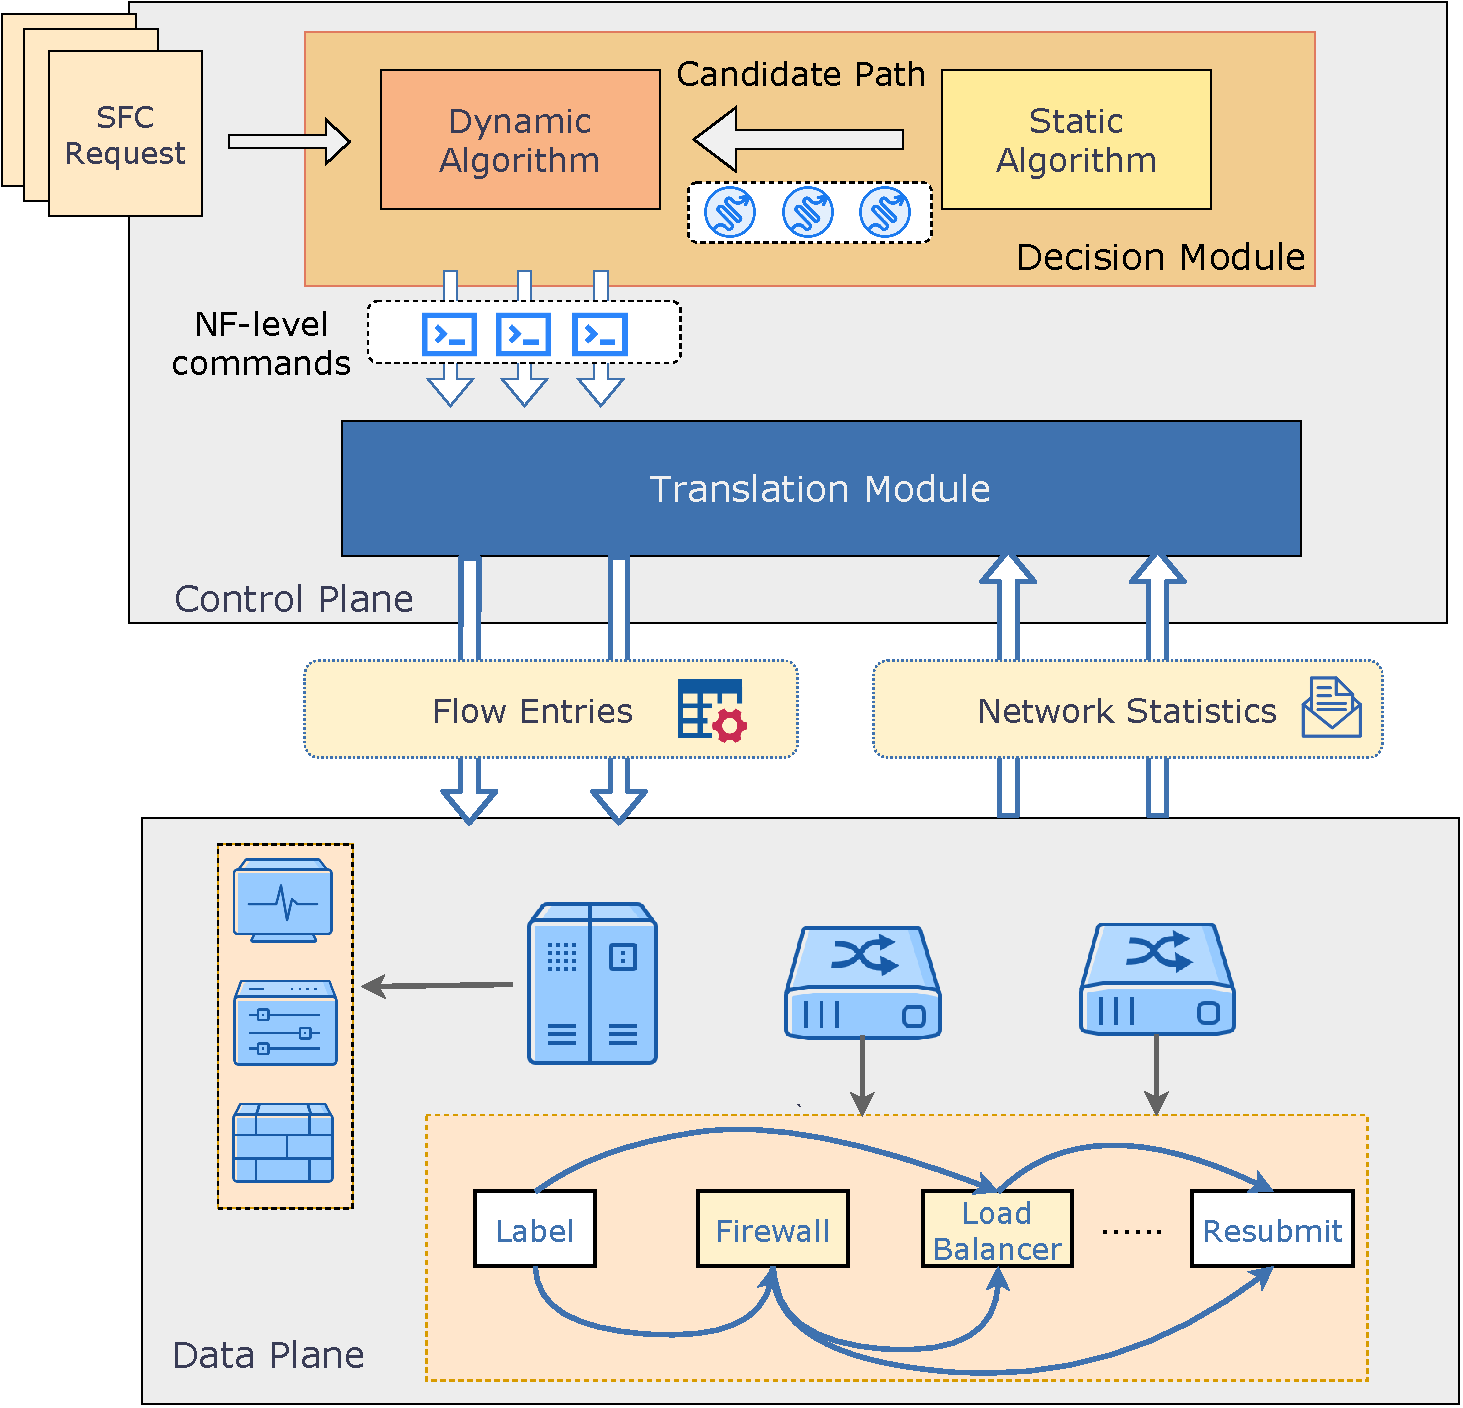
\includegraphics[width=0.85\linewidth]{src/arch.pdf}}
\caption{System architecture overview}
\label{architecture}
\end{figure}
 
\section{Background}

\subsection{P4 Langauage}
P4\cite{bosshart2014p4} is a domain specific language, which describes the packet processing pipeline of data plane device.  P4 was proposed as a target-independent abstract model for packet processing, in which the programmer does not need to know the specifications of the underlying forwarding device in terms of the device type or technologies(e.g., ASIC, FPGA, CPU). Therefore, the programs written in P4 language, can be mapped to several kinds of devices. 

A P4 program is composed of headers, parsers, metadata, match-action tables, and control flows. A match-action table matches the specified packet header fields and selects an action to execute. We use match-action tables to compose NF implementations or as a flow classifier. Metadata in P4 program is used to exchange processing information between tables, and a control flow specifies the order and logic of table processing. P4 community provides sound ecosystem, with its own compiler, P4C, to load the program to target devices and its southbound API, P4Runtime,  to expose the device capabilities for operators to populate rules at runtime. Leveraging these comprehensive building blocks provided by P4, we are able to rapidly build and deploy custom high-level applications.

\begin{table}[t]
\caption{Comparison of Programmable Data Planes}
\begin{center}
\begin{tabular}{|c|c|c|c|}
\hline
\textbf{Platforms}&\textbf{Expressiveness}&\textbf{Simplicity}&\textbf{Performance}\\
\hline
CPU& \checkmark & \checkmark & $\times$ \\
\hline
OpenFlow& $\times$ & \checkmark & \checkmark  \\
\hline
FPGA& \checkmark & $\times$ & \checkmark \\
\hline
P4& \checkmark & \checkmark & \checkmark\\
\hline
\end{tabular}
\label{comparison}
\end{center}
\end{table}

\subsection{Hardware Offloading}
Recently, some works proposed to offload certain network functions to programmable data plane to address the performance problem of NFV. OpenState was the first to propose to implement advanced stateful applications by extending match-action paradigm of Open Flow\cite{Bianchi2014}. However, OpenState hasn't mentioned the rationale to support and organize multiple applications. Besides, without the extension of OpenState, OpenFlow itself provides limited support for stateful operation and is not able to keep states inside the data plane.
On the other hand, FPGA-based SmartNIC is another available option to offload VNF\cite{Sun2017}\cite{Li2016}\cite{Pontarelli2019} \cite{sun2017hyper}. Microsoft proposed ClickNP, which deployed FPGA-based SmartNICs in their datacenters in order to save CPU usage and reduce the amount of traffic on a server’s PCIe bus, thus improving a network function’s packet processing latency by more than an order of magnitude\cite{Pontarelli2019}. However, programming a Smart-NIC requires proprietary hardware program expertise, which makes it difficult to support new features in existing devices.

As a target-independent domain-specific language, P4 offers great programmability by allowing network engineers to customize their protocol using descriptive language. As in Table \ref{comparison}, P4 maintains a good balance between expressiveness and simplicity. 
Meanwhile, P4 allows to maintain information in the data plane during runtime based on its register data structure, offering the potential to offload more advanced network functions. 
In addition, the advent of barefoot tofino ASIC provides the feasibility of deploying VNF on physical hardware device.
%Meanwhile, the routing loop problem will be resolved by on-path deploy.
%Some recent work recognized the benefits of combining hardware and software to achieve both high performance and flexibility of NFV. HYPER provides the ability to support a variety of VNFs based on state of the art programmable hardware and software platforms, and introduces a SLA-aware service chaining algorithm to provide better quality of service.

\subsection{Service Chaining Solutions}
To cope with different service chain requirements, a critical problem rooted inside programmable data plane is to organize and manage NFs to support multiple service chains. 

A natural strawman solution for service chaining is to implement one or more service chains in a single programmable switch. P4Visor proposed to improve this solution by merging multiple PDP programs in a single switch through a combination of compiler optimizations and program analysis-based algorithms. 
Although more flexible than the navie solution, the scheme still lacks reusability and scalability. For each slightly changed request, a service chain entity will be installed and occupy all or half of the switch.

Some researchers \cite{hancock2016hyper4} \cite{zhang2019hypervdp} offers another way to orchestrate NFs by leveraging match-action tables to simulate control logic, thus virtualizing PDP and realizing real-time reconfiguration. However, these solutions have brought in the problem of resource waste. For a simple service chain example firewall$\rightarrow$switch$\rightarrow$router, Hyper4\cite{hancock2016hyper4} and HyperVDP\cite{zhang2019hypervdp} use 7x and 3.2x table resources respectively, without mentioning other resources such as metadata.

ClickP4 offers the potential of dynamically combining features on programmable switches via tagging flows in front of performing NF logic. But it is limited to program decomposition and feature orchestration without focus on NF implementation model and schedule scheme for multiple switches.


\begin{figure}[t]
\centering  
\subfloat[initial flow table]{  
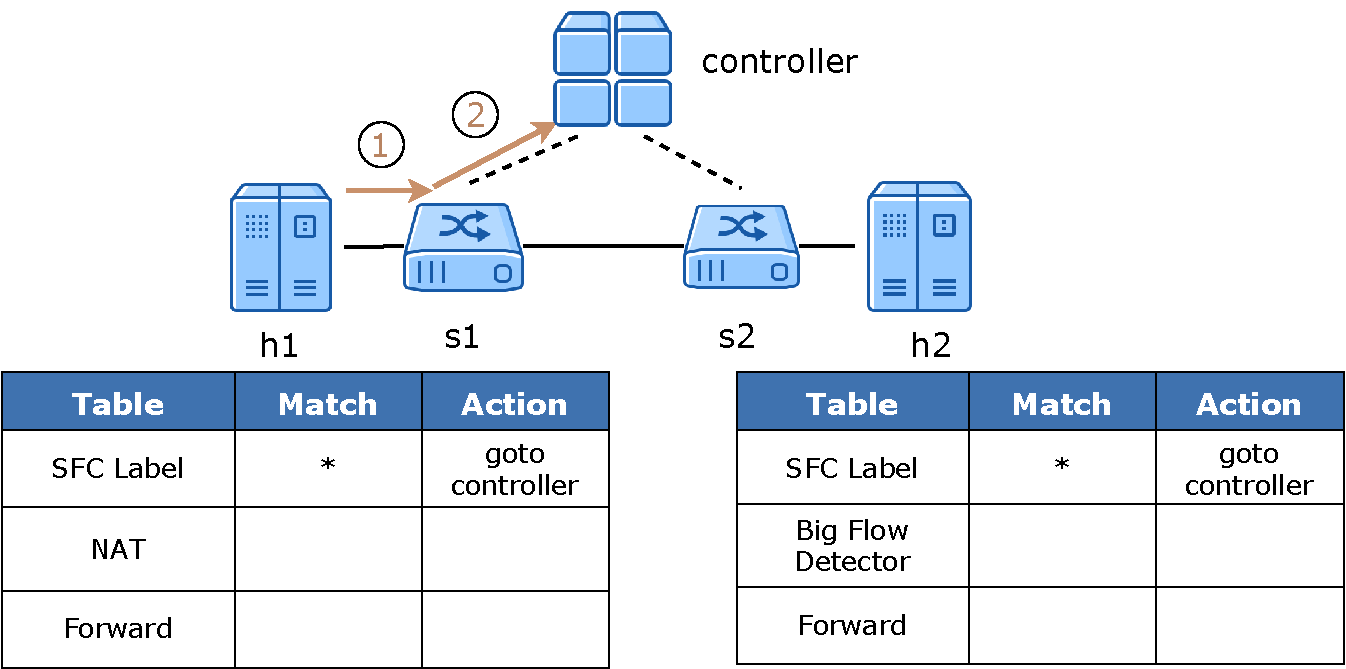
\includegraphics[width=0.45\textwidth]{src/suba.pdf}}  
\label{1a}\hfill  
\subfloat[system workflow]{  
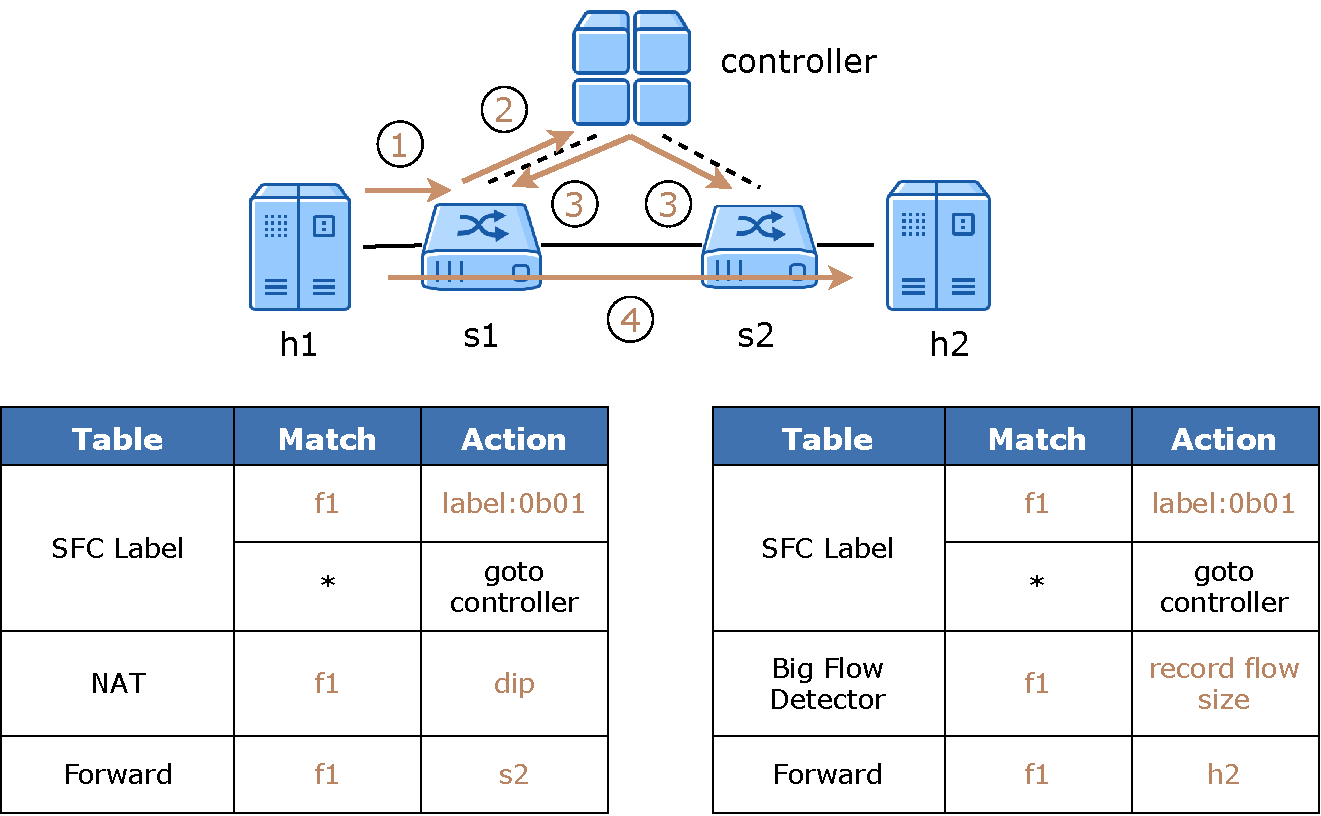
\includegraphics[width=0.45\textwidth]{src/subb.pdf}}  
\label{1b}\\
\caption{Figure a depicts the flow table of switch 1 and switch 2 when receiving the first packet of incoming flow flow1. The controller receives packet and thus deploy corresponding flow rules in s1 and s2 as in figure b. The green rules means that this rule is matched.}  
\label{arch}  
\end{figure}

\section{System Overview}
System architecture consists of HNF instances in data plane and control plane designs for NF management and flow allocation. System workflow is introduced through packet processing procedure.

\subsection{Data Plane}\label{AA}
Data plane is responsible for forwarding packets and supporting HNF instances. In STH, we use two kinds of models to represent hardware-based NF implementation. 1) Stateless NF leverages match-action tables to execute required actions on specific flow. 2) As for stateful NF, we adopt the Finite State Machine paradigm simulated by state-condition-action pipeline, thus keeping state access and transition inside data plane. 

In data plane, multiple HNFs are implemented in a certain order. The specific order and type are determined by the P4 program written by the operator.
To fulfill the diverse service chain requirements of flows, HNFs intra- or inter-switches must be dynamically composed. We utilize labels to identify the HNF sequence to go through in the current switch. In this way, flows is able to jump over HNF instances depending on controller decision.
As introduced before, maintaining state consistency is a significant task for data plane. To address this issue, indexes for stateful units access of HNFs are installed by controller along with the labels.

Although the primitives provided by the programmable data plane can support a large part of the operations of NF, there are still several NFs that are not suitable for hardware implementation. After research, we found NFs with too complex operations which are not supported by hardware capabilities, such as DPI, Carrier Grade NA(P)T, are not fully supported by the programmable data plane for the operation of packets. 
In addition, considering that hardware resources are more scarce than software resources, when hardware resources cannot guarantee NF deployment requirements and basic forwarding requirements, it is still necessary to use VNF deployment on general COTS equipment.


\subsection{Control Plane}\label{BB}
The control plane is composed of three modules: decision module and translation module.

The decision module is responsible for specifying NF instances for each incoming flow. The rationale of flow allocation is to ensure that switches in path still has sufficient remaining flow space for packets forwarding after installing HNF rules, preserving scalability and flexibility of system. To this end, a two-stage algorithm is contained in decision module that combines static path construction algorithm and dynamic path selection algorithm.
The static path construction algorithm takes the flows' demands  file as input and calculates the optimal set with k alternative paths for each flow. The candidate set are obtained under a some performance criterion such as having the large capacities or having the shortest number of hops. The static algorithm is only called when the topology changes.
 The dynamic path selection algorithm selects the currently optimal path from the candidate set through dynamic evaluation criteria (such as link load) combined with the impact of the resubmission operation on the system when new flows arrive. 
 The input requirements file defines all possible requests. A request is defined as $<$source IP, destination IP, NF sequence$>$. For the simplicity of implementation, our system uses source-destination IP pairs to determine a flow, but it can be easily extended to other flow definition forms. In the request file, operators can customize NF parameters, such as the threshold of Big Flow Detector.
%solve the problem of choosing the optimal instance for each request to reduce the extra use of ow table space as much as possible, 

%NF manager is responsible for managing state and NF migration. NF manager module provides state location allocation and retrieve for flows to access the right state. Since HNF is  initiated and deleted along with the flow, NF manager module merely pays extra attention to the issue of state acquisition and allocation to new instances during NF migration.

Translation module simplifies operator workflow by providing primitives for decision module to translate NF-level commands into flow table rules of data plane.

\subsection{A Packet's Life}
We then describe the packet processing procedure of STH.
As shown in \ref{arch}, the control flow ofSFC table, forward table and corresponding NF table will be proactively installed in data plane as the processing logic of HNF framework.
Assume a request flow $f1$ with SFC requirements NAT$\rightarrow$Big Flow Detector arrives at switch $s1$, the system will process it through 4 steps.
(1) After the first packet of flow $f1$ enters the edge switch, according to Fig. \ref{1a}, it will first be sent to the controller via match miss of the SFC label table since label allocation entries of this flow havnt't been installed yet.
(2) After receiving packet-in, the controller will run a dynamic selection algorithm to choose an optimal path with requested NFs for the flow. The specific detail of the algorithm is described in Section-5. 
(3) The controller will install rules of SFC table, forwarding table and NF table for $f1$ on switches along with the selected path.
(4) Subsequent packets of $f1$ will match flow table rules at $s1$ and $s2$, and be correctly forwarded to destination  with service chain requirements accomplished.


\begin{figure}[t]
\centerline{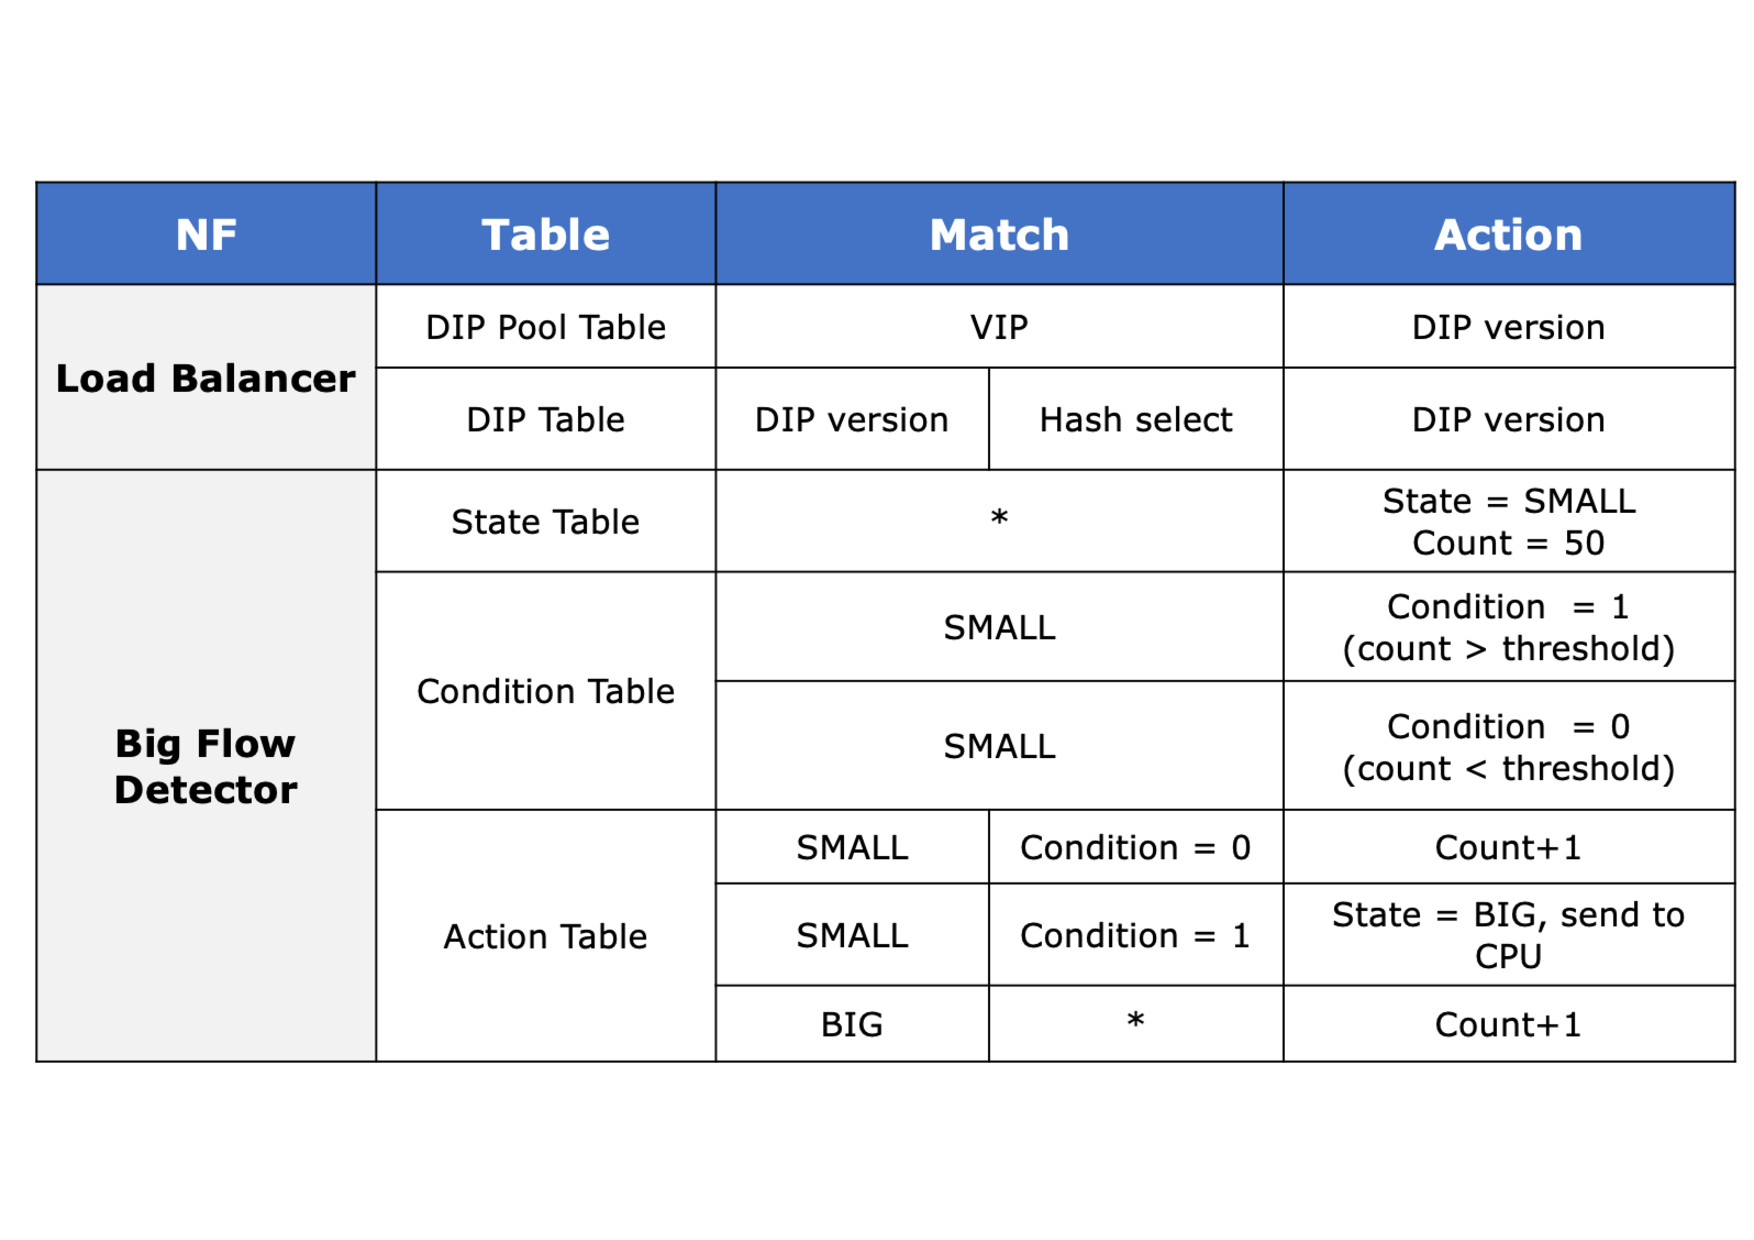
\includegraphics[scale=0.3]{src/flow.pdf}}
\caption{Flow Table Implementation of Load Balancer and Big Flow Detector}
\label{flow}
\end{figure}


%\begin{figure}[t]  
%\centering  
%\subfloat[]{  
%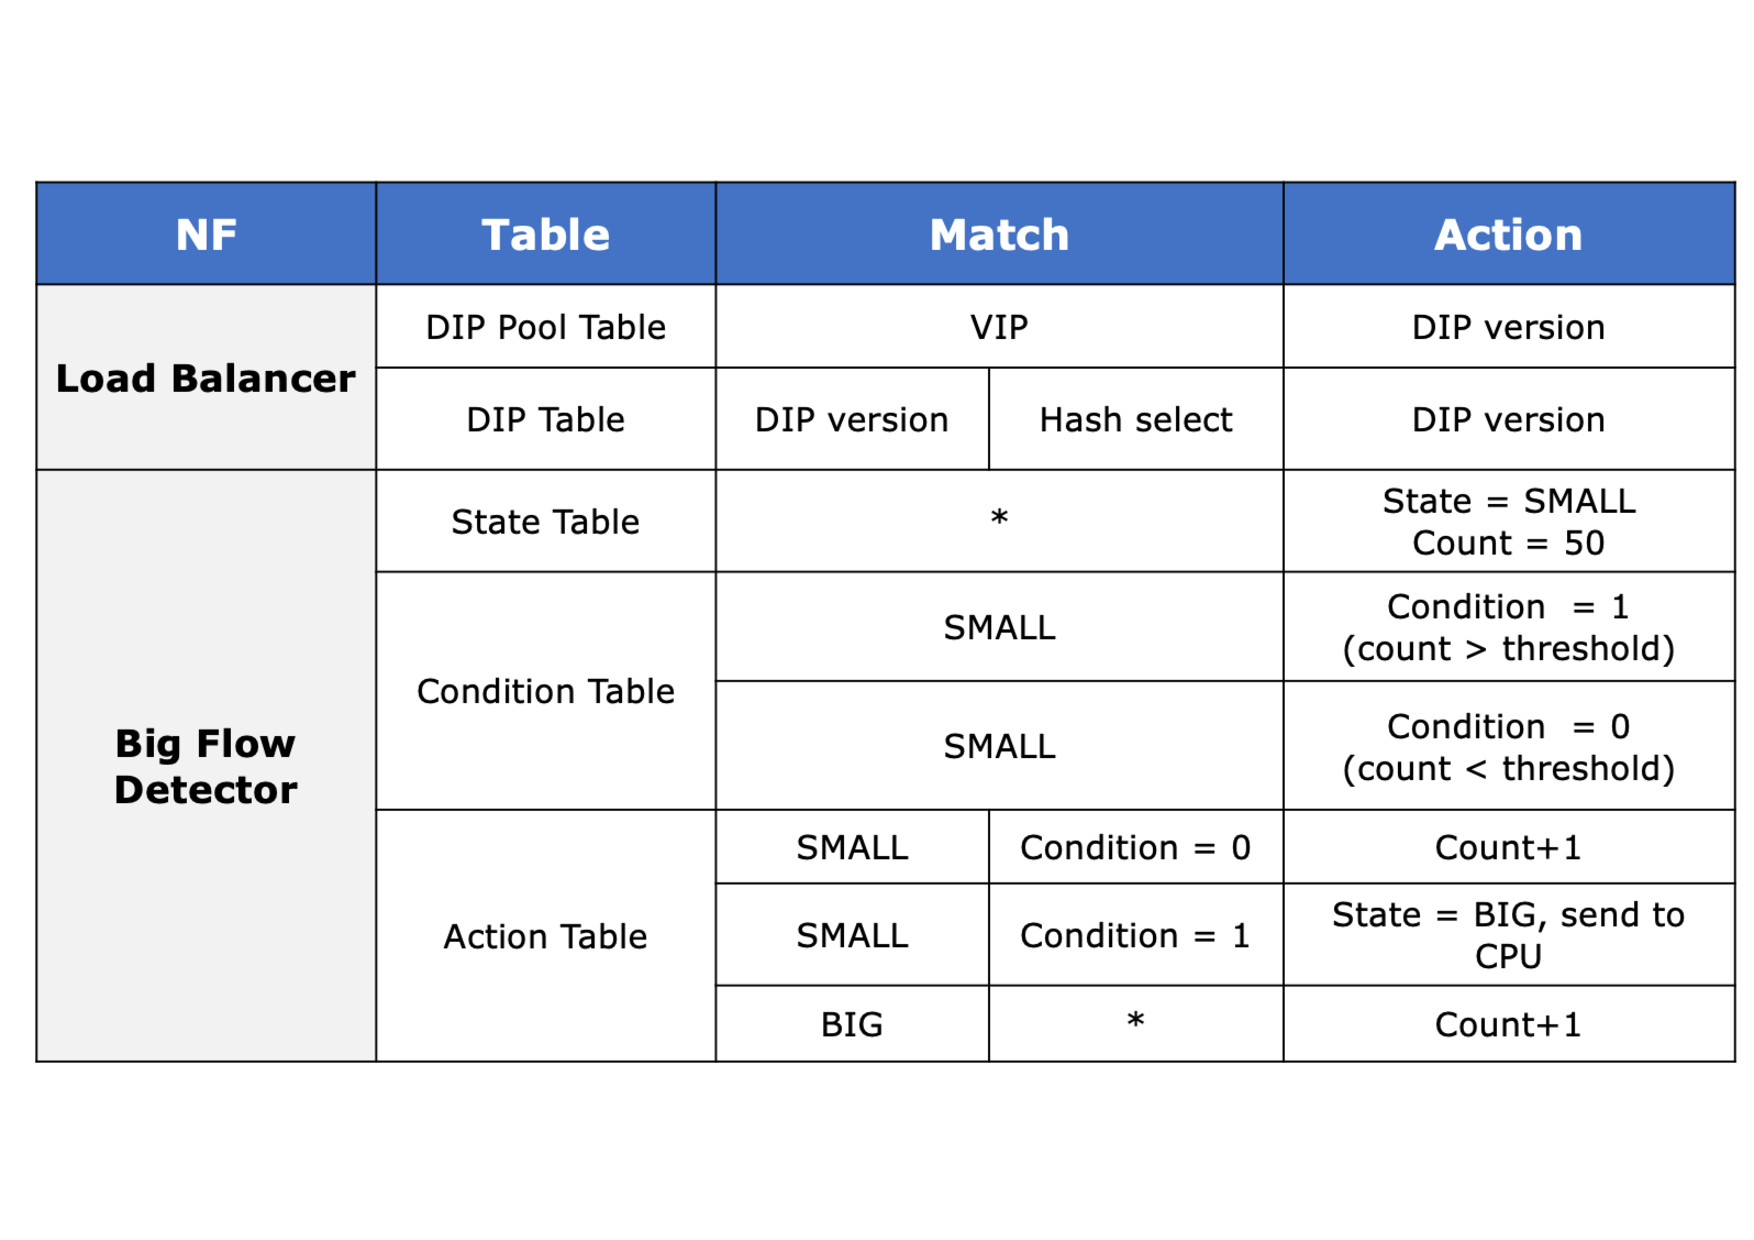
\includegraphics[width=0.45\linewidth]{src/flow.pdf}
%\label{flow}
%\subfloat[]{  
%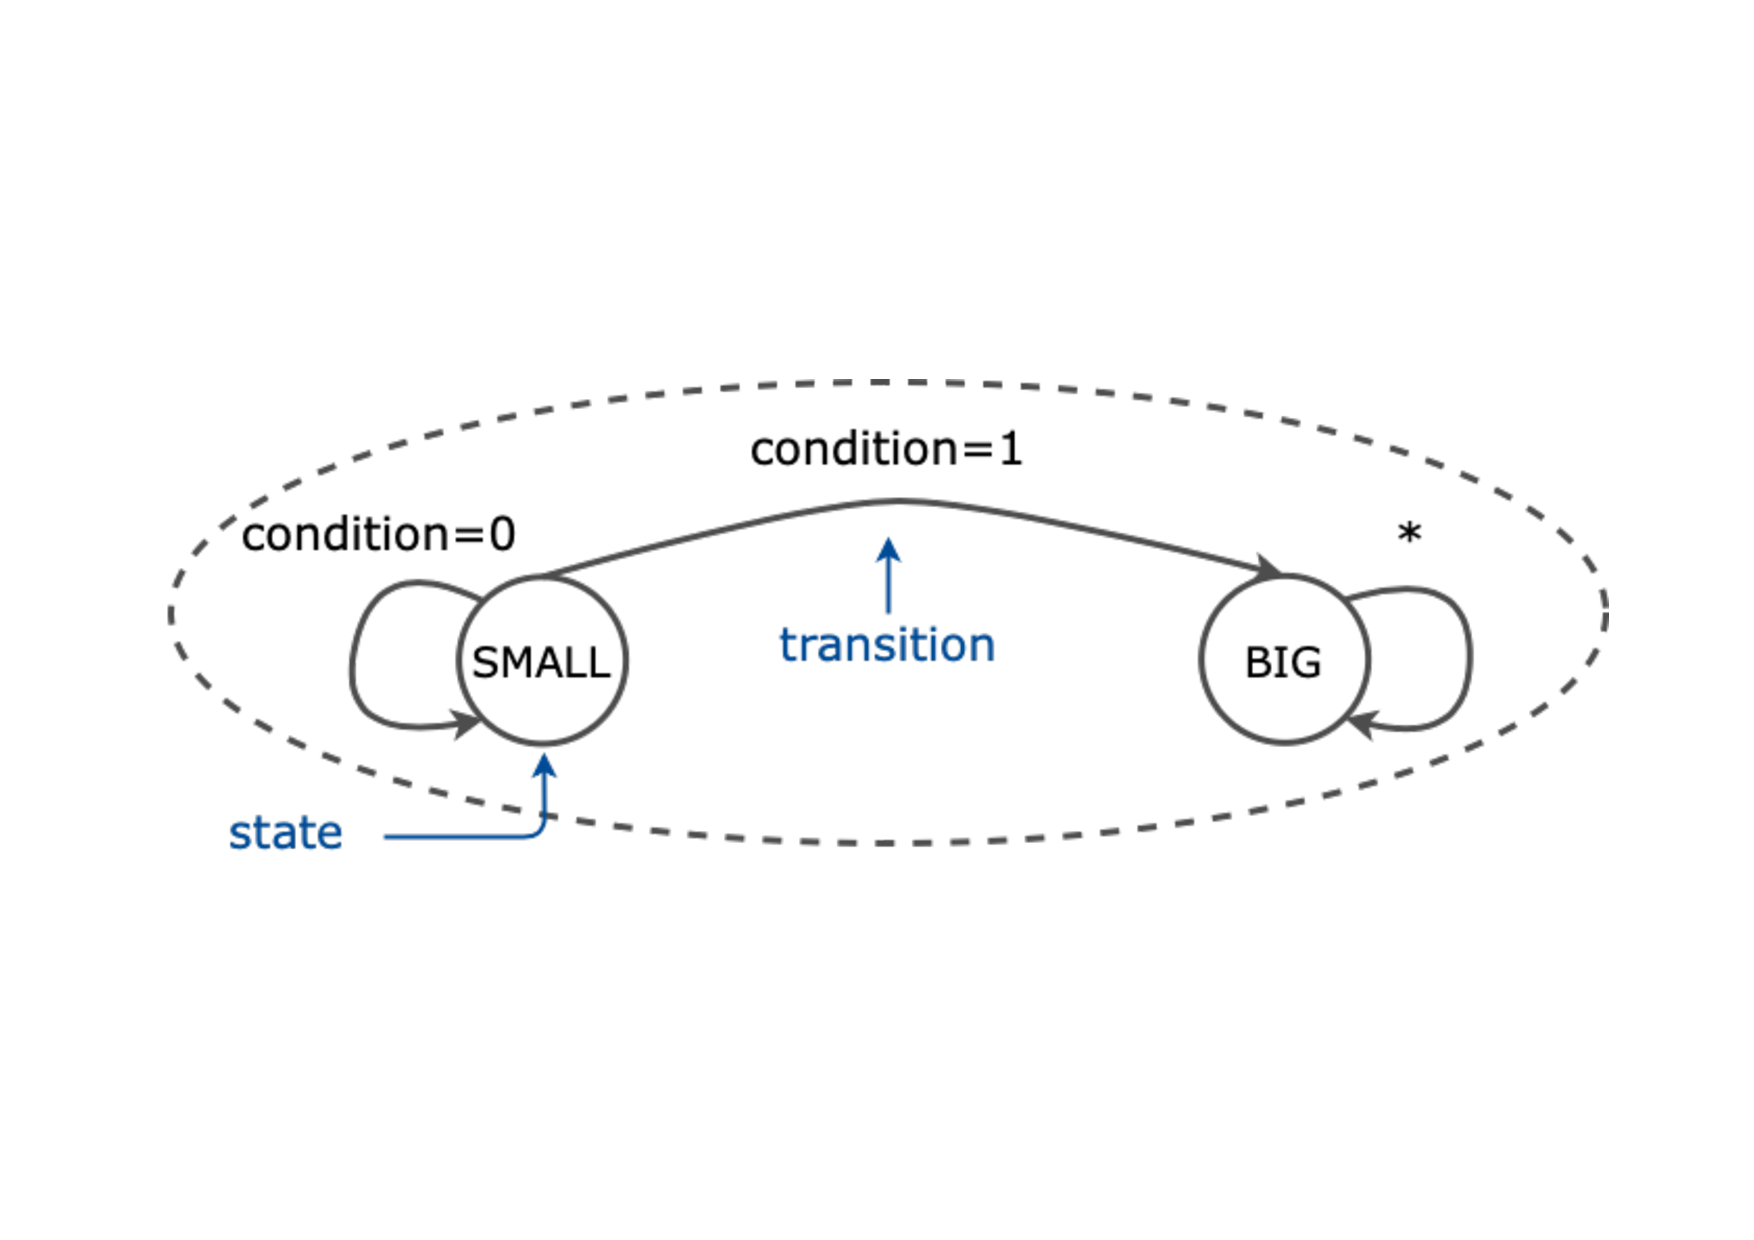
\includegraphics[width=0.45\linewidth]{src/fsm.pdf} 
%\label{fsm}\\
%\caption{Flow Table Implementation of Load Balancer and Big Flow and Finite State Machine Example}  
%\label{3}  
%\end{figure} 

\section{Data Plane Design}
Data plane supports the dynamic HNF framework, which could be divided into three parts: NF implementation paradigm, state management and dynamic chaining.
\subsection{NF Implementation Paradigm}
Hardware-based NFs in PDP could be classified into two types: stateful NF and stateless NF, and we propose two models to better illustrate their features.

(\expandafter{\romannumeral1}) Stateless NF is implemented via a series of Match-Action Table (MAT) units. We use Layer-4 Load Balancer as an example. Stateful layer-4 (L4) load balancers scale out services hosted in cloud datacenters by mapping packets destined to a service with a virtual IP address (VIP) to a pool of servers with multiple direct IP addresses (DIPs or DIP pool). 
To complete this task, two sequentially placed tables are needed as in Fig.\ref{stateless}, where the first one allocates DIP pool labels by matching VIPs, and in the second one, flows finally get DIP with DIP pool label and hash result (to randomly select DIP from DIP pool).


(\expandafter{\romannumeral2}) Stateful NF requires information generated during processing the former packets of the same flow\cite{Gember-Jacobson2015}. As Fig.\ref{fsm} shows, stateful NF can be represented by the Finite State Machine. 
Each node represents a different state, and each arrow represents the transition between states. 
When condition on the shoulder are met, state transition will be performed. As shown in the example of Big Flow Detector, when number of recorded packets exceeds the threshold, state will move to BIG and the corresponding flow should be reported to the controller.

To simulate the logic of FSM in P4 switch, we use three types of tables to process packets, called state table, condition table and action table. 

\begin{itemize}
\item \textbf{State table} is responsible for obtaining corresponding state of the flow. Each HNF has its own stateful units as register array in programmable switch. In this example, SMALL and BIG states are respectively represented as 0 and 1. In addition, flow will also need to count packets to compare with threshold. Thus, we concatenate state and packet count information together, e.g. $1100100$ means state SMALL with packet count 50 as in Fig.\ref{bfd}. After fetching state index of this HNF in SFC table, the packet will read and preserve state in its metadata.
%State can be accessed through hashing the certain fields of the packet header (i.e., 5 tuple, src and dst IP address).
\end{itemize}

\begin{itemize}
\item \textbf{Condition table} implements state transition logic in FSM. By conducting predefined calculations with metadata and threshold, we can obtain condition result and determine which state to go next. In the BFD example, if state is greater than threshold, the condition value will be set at 1, otherwise 0. The number of condition table entries is equal to the number of state transitions (arrows) in FSM model.
\end{itemize}

\begin{itemize}
\item \textbf{Action table} performs actions on both packet and state. State action allows modifying and rewriting state back to the register array, which will be obtained by the next packet. Packet action includes packet header modification or packet dropping. 
In this example, there are three different possible action. When flow state is small and condition is 0, it is still a small flow, we will just increment the counter; when the flow state is small and condition is 1, it represents that flow state transition happens, and packet will be sent to CPU for notification; When state is big, HNF will keep counting and waiting for controller instruction.
\end{itemize} 



\begin{table}[t]
\caption{Comparison between Hash and Controller Issue}
\begin{center}
\begin{tabular}{|c|c|c|c|}
\hline
\textbf{Trace}&\textbf{Hash Space}&\textbf{Collision Rate}&\textbf{Memory Used (KB)}\\
\hline
\multirow{5}{*}{univ1} & $2^{12}$ & $33.94\%$ & $0.5$ \\
\cline{2-4}
~ & $2^{14}$ & $10.49\%$ & $2.0$ \\
\cline{2-4}
~ & $2^{16}$ & $2.67\%$ & $8.0$ \\
\cline{2-4}
~ & $2^{18}$ & $0.81\%$ & $32.0$ \\
\cline{2-4}
~ & \textbf{controller issue} & $0$ & $5.8$ \\
\hline
\multirow{5}{*}{univ2} & $2^{14}$ & $22.30\%$ & $2.0$ \\
\cline{2-4}
~ & $2^{16}$ & $6.27\%$ & $8.0$ \\
\cline{2-4}
~ & $2^{18}$ & $1.81\%$ & $32.0$ \\
\cline{2-4}
~ & $2^{20}$ & $0.36\%$ & $128.0$ \\
\cline{2-4}
~ & \textbf{controller issue} & $0$ & $15.94$ \\
\hline
\end{tabular}
\label{hash}
\end{center}
\end{table}

\begin{figure}[t]
\centerline{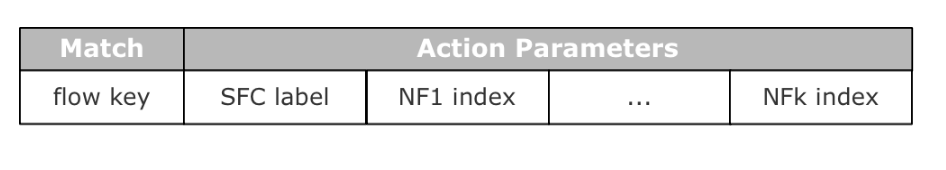
\includegraphics[scale=0.3]{src/sfc.png}}
\caption{SFC table implementation}
\label{sfc}
\end{figure}


\subsection{Service Chaining Design}
To identify diverse SFC path, we utilize SFC labels coding in one-hot form for each flow. A SFC label table is implemented ahead of all the HNF tables in every switch, entries of which are deployed by the controller. To enable reverse order of HNFs on a switch, resubmit operation provided by P4 platform that sends the packet back to the start of pipeline.

The length of SFC label is equal to $|SFC|+1$ ($|SFC|$ means length of HNF sequence in a switch). The $kth$ bit of SFC label in binary form indicates whether packets should pass the $kth$ NF ($k <|SFC|$). For example, on a switch with SFC Big Flow Detector $\rightarrow$ Firewall $\rightarrow$ Load Balancer installed, $0b0101$ indicates that corresponding flow needs to pass through Big Flow Detector and Load Balancer in sequence. 

In order to identify resubmission requirements, the highest bit of SFC label indicates whether resubmission is required. We add a resubmission table at the terminal of switch pipeline, with matching field set as flow key, and action parameter set as new flow label. 
The system now supports flow to go through pipeline for two times. But for situations that require multiple resubmissions, we can simply add an additional matching field of resubmit table to identify the times of resubmissions. However, since resubmission will impact system performance, it's not recommended to overuse resubmit operations. 


\subsection{State Management}
Operations of network functions usually involve stateful operations. State refers to information generated from operation of previous packet, which could be used to guide subsequent packets of the same flow. 

P4 platform provides stateful units (embodied as register array) with reading and writing API exposed to P4 program.
In a HNF instance, a series of stateful unit memories will be declared, with width equal to bits of state that needs to be stored, and length equal to the maximum number of flows that may pass through the function.

In order to enable the correctness of function, the data plane needs to ensure state consistency, that is, subsequent packets of the same flow access stateful units through the same index. There are two ways to ensure state consistency. 
The first one is to hash header fields of packets to get theirs HNF state indexes, thus packets of the same flow is able to get the same result.
However, hash collision is an unavoidable problem, leading to different flows operating on the same state, which interferes result correctness. Moreover, hash collision solutions including open addressing and separate chaining are hardware-friendly. 
The second way is for controller to issue state index through SFC table as in \ref{sfc}. Incoming flows will first have to go through SFC table and obtain the state index for all HNFs in need on this switch. Extra memory will be introduced through storing state index.

To evaluate these methods, we use two traces to compare collision rate and used memory under two schemes. The result is shown in \ref{hash}, the first four entries of each trace use hash function and the fifth one obtains state index issued by controller. 
Hash function shows a bad performance under two circumstances. Only when a larger space is given to stateful units (6.4x and 8.6x larger than memory used by table rules method) can hash collision rate be reduced to a relatively small range ($<1\%$).



\section{Control Plane Design}
The decision module uses a two-stage algorithm consisting of static and dynamic algorithm to construct SFC routing path for flows. 

%In a system with both software and hardware NF installed, the mapping algorithm should solve the problem of choosing the optimal instance for each request to reduce the extra use of flow table space as much as possible, thereby making the system more scalable.


\subsection{Problem Definition}
%When a new request arrives, it is necessary to map the requested VNFs to the underlying network infrastructure while ensuring service requirements and network overhead, that is, to map the virtual network function forwarding map to the physical topology. 
When a new request arrives, a forwarding path should be constructed meeting following rules: (1) NF sequences in order as requested is provided on the path. (2) nodes along the path have available remaining resources (flow table resources of switches and processing resources of servers) (3) links along the path have available remaining bandwidth. Meanwhile, in order to ensure network performance and avoid potential congestion, the shortest possible path should be selected on the basis of restrictions.

%In the P4 switch environment, the challenge of NF mapping mainly lies in how to use the limited switch flow table space resources to improve the performance of the entire system.

The data plane topology is modeled as an undirected graph $G=(V, N, E)$, where V, N and E denote the node set, NF set and link set respectively. Meanwhile, we model the incoming request to be deployed as $R=(N_r, v_{s}, v_{d}, b_r)$. $N_r$ denotes the required service chain of request $r$. Other attributes of request $r$ include source and destination node $v_{s}$, $v_{d}$, as well as initial data rate $b_r$. 

\begin{equation}
\min \quad w_{l} \cdot \frac{m_{l}}{l}+w_{r} \cdot \frac{m_{r}}{|r|}
\end{equation}

In order to improve performance of request while reducing the possibility of network congestion, we set the target of constructing forwarding path as Eq. (1), parameters of which are defined as: 

\begin{equation}
m_{l}=\sum_{i}\sum_{v, v^{\prime} \in V, v \neq v^{\prime}} t_{v, v^{\prime}} \cdot y_{N_{i}}^{v} \cdot  y_{N_{i+1}}^{v^{\prime}} \cdot \frac{b_{r}}{b_{v, v^{\prime}}}
\end{equation}

\begin{equation}
l = \sum_{i}\sum_{v, v^{\prime} \in V, v \neq v^{\prime}} t_{v, v^{\prime}} \cdot y_{N_{i}}^{v} \cdot  y_{N_{i+1}}^{v^{\prime}}
\end{equation}

\begin{equation}
m_{r} = \sum_{i=1}^{|r|-1} \sum_{v \in V_{s}} y_{N_{i}}^{v} \cdot y_{N_{i+1}}^{v} \cdot d_{N_{i}, N_{i+1}}^{v} 
\end{equation}


\setlength{\tabcolsep}{1mm}{
\begin{table}[t]
\caption{Network Model Notation}
\begin{center}
\begin{tabular}{p{60pt}p{180pt}}
\hline
\textbf{Notations}&\textbf{Description}\\
\hline
$N$ & The set of NFs within the network\\
\hline
$V$ & The set of nodes including switches $V_s$ and hosts $V_h$\\
\hline
$E$ & The set of links within the network\\
\hline
$N_r$ & Required SFC of request $r$\\
\hline
$b_r$ & Estimated data rate of request $R$\\
\hline
$c_{v}$ & Residual processing capacity of node $v$\\
\hline
$b(v, v^{\prime})$ & Residual bandwidth resources of link  $(v, v^{\prime})$\\
\hline
$x_{N_{i}}^{v}$ & =1 if NF $N_{i}$ is implemented on node $v$\\
\hline
$d_{N_{i}}^{v}$ & =1 if NF $N_{i+1}$ is implemented before  $N_{i}$ on node $v$\\
\hline
$y_{N_{i}}^{v}$ & Binary variable to designate NF $N_{i}$ is assigned to node $v$\\
\hline
$t_{v, v^{\prime}}$ & Binary variable to designate result path $p$ contains link $(v, v^{\prime})$\\
\hline
\end{tabular}
\label{notation}
\end{center}
\end{table}
}

The optimization goal is divided into two parts: 
1) In order to guarantee the quality of service for request, the link bandwidth utilization should be minimized, denoted as $m_l$ in Eq.(2), where $t_{v,v^{\prime}}$ indicates whether $(v, v^{\prime})$ is included in the optimal path $p$, $y_{N_{i}}^{v}$ indicates whether NF $N_{i}$ is allocated to node $v$, and the bandwidth utilization ratio is obtained by dividing the data rate $b_{r}$ by the remaining bandwidth $b(v, v^{\prime})$ of link $(v, v^{\prime})$.
2) Since resubmission operation(i.e., packets return to the beginning of current pipeline) is allowed in the system , which brings flexibility while affecting the throughput of both request and corresponding switch.  Therefore, we added a second part to the optimization goal to weigh the impact of path stretching and resubmission. 
$m_{r}$, times of submissions on the entire service chain of request $r$, is calculated by Eq.(4), where $d_{N_{i}, N_{i+1}}^{v}$ indicates whether $N_{i+1}$ is implemented before $N_{i}$ on switch $v$.

In the optimization goal, metrics are respectively normalized ($m_l$ divided by the total length of path in terms of links $l$ in Eq.(3), $m_r$ divided by the length of service chain) to evaluate them from the same dimension. Since $m_l$ and $m_r$ have different effects on performance under different network circumstances, we use two weights $w_l$ and $w_r$ to change the importance of these metrics in path construction.
 


\begin{equation}
t_{v, v^{\prime}} \cdot b_{r}<b_{v, v^{\prime}}, \quad \forall v, v^{\prime} \in V, (v, v^{\prime}) \in E
\end{equation}

\begin{equation}
\sum_{i} y_{N_{i}}^{v} \cdot m_{i}<c_{v} \quad \forall v \in V_{s}
\end{equation}

\begin{equation}
\sum_{i} y_{N_{i}}^{v} \cdot p_{i}<c_{v} \quad \forall v \in V_{h}
\end{equation}

Eq. (5) describes the traffic load constraints on each link $v, v^{\prime}$. Eq. (6) and Eq. (7) state resource capacity on each switch $v_s$ and each server $v_h$, where $m_i$ and $p_i$ denote memory and processing resource consumption of NF $i$ respectively.

\begin{equation}
\sum_{v^{\prime}, \tilde{v} \in V_{s}, v \neq \tilde{v}}\left(t_{v, v^{\prime}} \cdot t_{v, \tilde{v}}+t_{v^{\prime}, v} \cdot t_{\tilde{v}, v}\right)=0 \quad \forall v \in V
\end{equation}

Eq. (8) defines an important problem of loops in path, i.e., traffic passing through the same switch twice, resulting in traffic routing conflicts. For example, as in Fig. \ref{construct}a, for a flow with path: s1 $\rightarrow$ s2 $\rightarrow$ s1 $\rightarrow$ s3, routing entries of traffic on s2 would conflict, leading to wrong destination.

It should be noted that the loop on switches directly connected with software-NF service installed server is not within the limit. Because it is easy to install a control logic on directly connected switch that identifies and tags the traffic from the server to distinguish and forwards traffic depending on the tag.

\begin{equation}
\sum_{v \in V} y_{N_{i}}^{v}=1 \quad \forall i \in \left[1, |r|\right]\end{equation}

\begin{equation}
\sum_{v \in V} \operatorname{t}_{v_{s}, v}=1 \quad \sum_{v \in V} t_{v, v_{d}}=1
\end{equation}

\begin{equation}
y_{N_{i}}^{v}=0, \quad \text{if} \quad x_{N_{i}}^{v}=0
\end{equation}

\begin{equation}
\sum_{v^{\prime} \in V_s} (t_{v, v^{\prime}} + t_{v^{\prime}, v}=2), \quad \text{if} \quad y_{N_{i}}^{v}=1 \quad \forall v \in V
\end{equation}
Eq. (9) requires that each NF is only installed once, while Eq. (10) defines the start and destination of path. Eq. (11) and Eq. (12) ensure the correctness of variable $y_{N_{i}}^{v}$ and $t_{v, v^{\prime}}$.

In order to quickly respond to dynamic traffic, we need a heuristic algorithm for path construction. However, as a naive method, it is necessary to construct a multi-stage forwarding graph, and then use the shortest path algorithm to select the optimal path. 
Its time complexity is $O(N^2)$, growing with the total number of NF nodes in every stage, which is not conducive to rapid response to traffic. Therefore, we propose a two-stage algorithm to solve this problem.


\subsection{Static Path Construction Algorithm}
In order to reduce the workload of the dynamic algorithm, the candidate path set will be calculated from static algorithm stage as the input of dynamic algorithm. 
The static algorithm is only called when the topology is constructed or changed. Since realtime link load statistics cannot be obtained in static algorithm, we set the optimization goal in this stage as the weighted sum of path distance and resubmission times. The dynamic algorithm will evaluate paths according to link load ratio in realtime.

For all the requests defined in requirements file (introduced in section 3), we use the static path construction algorithm to select the top-k-shortest path as Algo. \ref{construction}.

At first, an NF forwarding graph based on the topology graph and SFC request is constructed.
The forwarding graph contains n + 2 stages (n is the length of SFC requirement). The first stage and the last stage are the source and destination nodes of the flow. The remaining nodes in each stage are the switches or hosts with corresponding NFs installed. The edge of the forwarding graph is assigned with the weighted sum of the distance of the shortest path between two nodes and resubmission times, which can be obtained by collecting network topology and request information. The procedure is presented in Fig. \ref{example}a, one of the request is depicted in the figure with the SFC request: B$\rightarrow$A$\rightarrow$D.

Next, we use the top-k-shortest path algorithm (i.e., Yen's algorithm) to obtain the set of the first k shortest paths. 
Since the path set obtained may contain routing loops, more paths than required are calculated from the KSP algorithm (i.e., set the parameter to $2k$), and then filter the paths in order. Paths that do not contain loops can be added candidate set, the algorithm stops when the size of candidate set reaches $k$.


\begin{algorithm}[t]
\KwIn{Network Topology Graph $G=(N, V, E)$, Request $R$}
\KwOut{NF-Forwarding Graph $g$ and Path Set $P$}
Step 1: Construct Forward Graph
$g.add(v_s)$

\For{$i \leftarrow 1$ \KwTo $|N_r|+2$}{
	\If{$v \in  N_{i}.nodes$}{
		$g.add(v)$\;
		\For{$j \in  N_{i-1}.nodes$}{
			$g[j][v] = w_{l} \cdot d[j][v] + m_{r} \cdot w_{r}$
%			w_{l} \cdot \frac{m_{l}}{l}+w_{r} \cdot \frac{m_{r}}{|r|}
		}
	}
}
Step 2: Get Candidate Path Set

$P^{\prime} = KSP(graph, k*2)$

\For{path $p \in P$}{
	\If{!p.containsLoop()}{
		$P.add(p)$\;
		if(P.size==k) \quad break;
	}
}
\caption{{\bf Static Path Construction Algorithm} \label{construction}}
\end{algorithm}


%\begin{figure}  
%\centering  
%\subfloat[]{  
%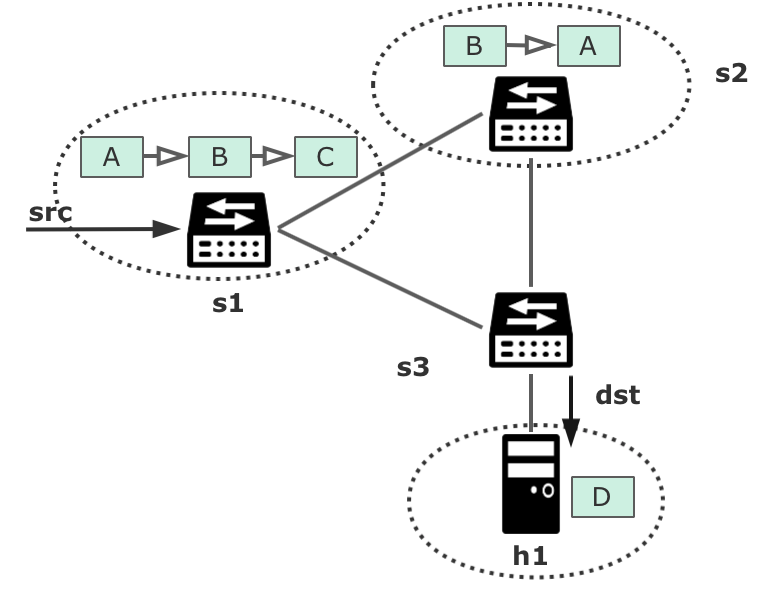
\includegraphics[width=0.45\linewidth]{src/subc.png}}  
%\label{one of the requests in network topology}
%\subfloat[]{  
%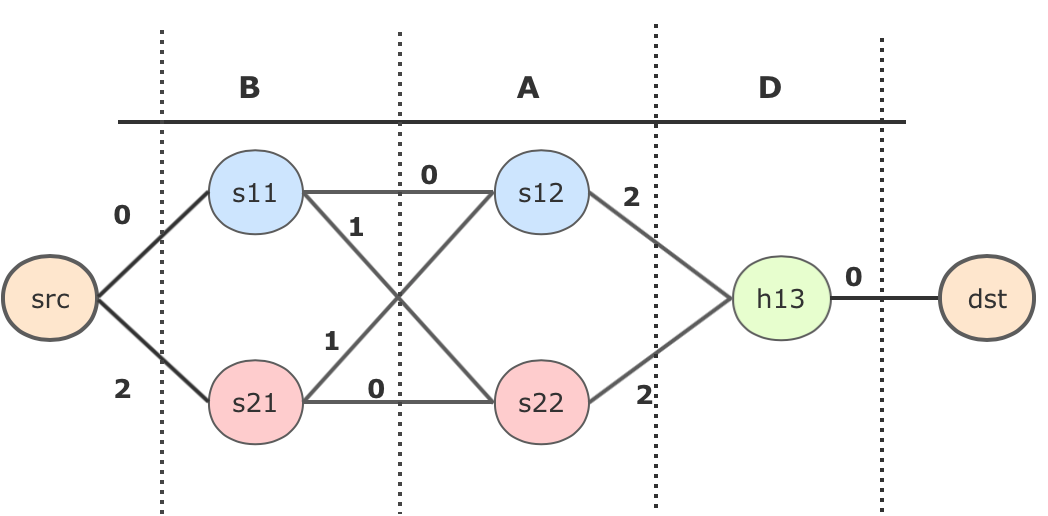
\includegraphics[width=0.45\linewidth]{src/subd.png}}  
%\label{2b}\\
%\caption{Figure 7a is the network topology with hardware and software NF instances installed and figure 7b is the constructed forward graph for one of the request.}  
%\label{construct}  
%\end{figure} 

\begin{figure}  
\centering  
\subfloat[one of the requests in network topology]{  
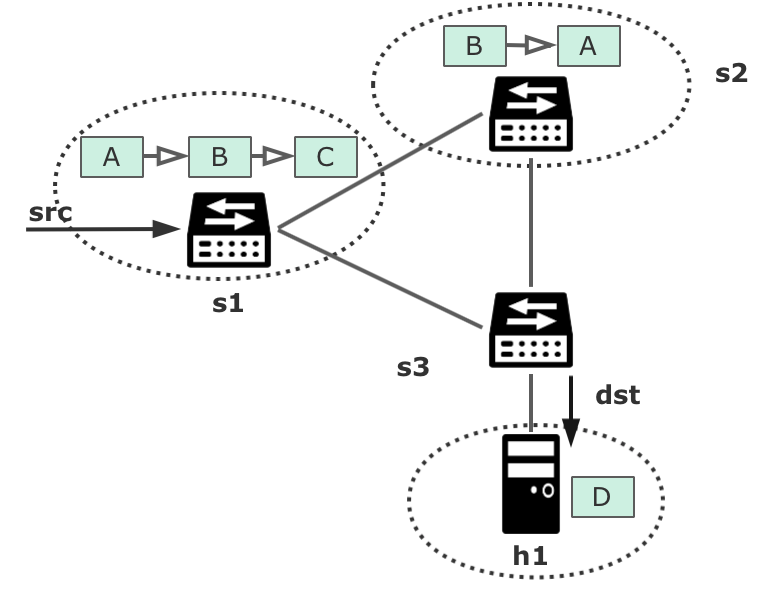
\includegraphics[width=0.7\linewidth]{src/subc.png}}  
\label{2a}\hfill  
\subfloat[constructed graph by algorithm]{  
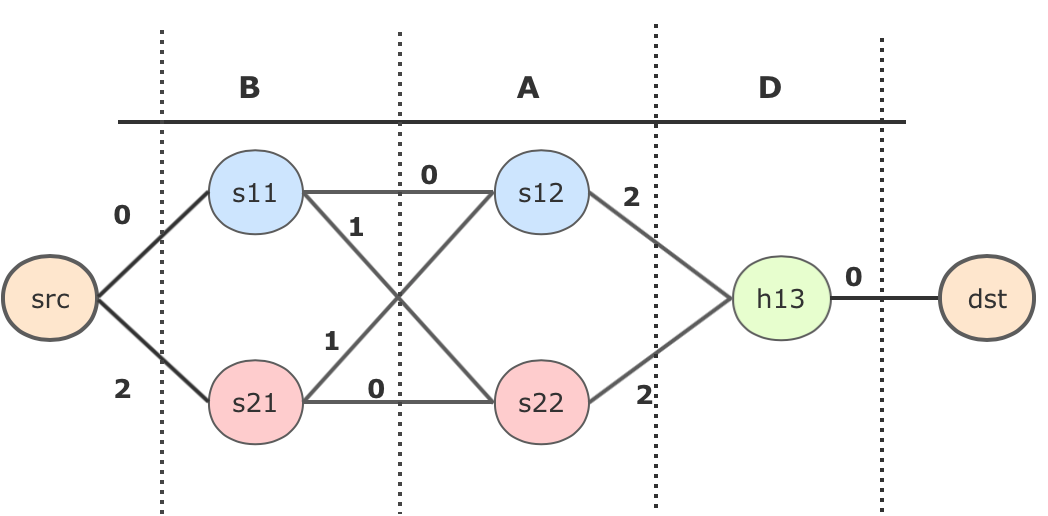
\includegraphics[width=0.7\linewidth]{src/subd.png}}  
\label{2b}\\
\caption{Figure 5a is the network topology with hardware and software NF instances installed and figure 5b is the constructed forward graph for one of the request.}  
\label{example}  
\end{figure} 



\subsection{Dynamic Path Selection Algorithm}
When the first packet of each request is forwarded to the controller, dynamic path selection algorithm will be activated to select the optimal path from candidate sets considering cumulative link load.

 As shown in Algorithm 2, the program will first read candidate path set from static algorithm. In order to avoid network congestion and further improve network performance, we set the metrics as cumulative sum of link load ratio (i.e., data rate divided by available bandwidth). 
 Thus, for each candidate path, restrictions of node capacity and link capacity along the path is first check to guarantee feasibility. Then, an optimal path in terms of link load usage is selected after traversing candidate set.
 The time complexity of dynamic path selection algorithm is $O(n)$ in terms of number of candidate path, which is a tolerable delay for packets.
% In order to minimize the extra use of flow table space, we define the metrics as the weighted sum of the cumulative sum of the bandwidth utilization of eacxh link on the path and the impact of resubmission. We quantify the impact of resubmission as the times of resubmissions in the entire path. Finally, select the one with the smallest metrics from all paths.


\begin{algorithm}[h]
\KwIn{Candidate Path Set P of Request R}
\KwOut{Optimal Path $p^\ast$ of Request R}

\nl minimum metrics $min = MAXIMUM$\;

\For{path $p \in P$}{
	\For{edge $e \in p$}{
			\If{$l[e] <= b_{r}$ or $c_{e.src} <= m_r$}{
				break;
			}
			\If{$m_l < min$}{
				$min = m_l$\;
				$p^\ast = p$
			}
	}
}
\caption{{\bf Dynamic Path Selection Algorithm} \label{Dynamic}}
\end{algorithm}



\section{Evaluation}
We have evaluated the system on both a software (Bmv2) and a hardware (Barefoot Tofino) programmable data plane about performance and overheads of hardware offloading, as well as performance of two-stage NF mapping algorithm. 

\subsection{Performance Benefits and Overheads of PDP}
\textbf{Experiment Setup}. On the (Barefoot Tofino) target, we implemented the following NFs: NAT, Firewall, Load Balancer, Stateful Firewall, Port Knocking Firewall and Big Flow Detector. Due the limitation of hardware devices on stateful actions, we made a little modifications on stateful HNF models by combining reading, comparing and writing HNF state into a single register action, thus avoiding conflicts. 
To evaluate the performance of hardware HNF from common NFV solutions, we build two chains: stateful chain of Port Knocking Firewall 	$\rightarrow$ Stateful Firewall 	$\rightarrow$  Big Flow Detector and stateless chain NAT 	$\rightarrow$ Firewall 	$\rightarrow$ Load Balancer, and use Ixia Tester to generate packets and analyze collected information. Throughput and hardware overhead(caused by HNF) are considered to evaluate hardware offloading scheme. We also evaluated the impact of multiple flows (1 - 1000) and the extra costs caused by dynamic chaining framework. As for software platforms, we utilized OpenNetVM to collect needed information.

\textbf{Performance}.

\textbf{Dealing with massive flow}.

\textbf{Hardware Overheads}.


\begin{figure}  
\centering  
\subfloat[]{  
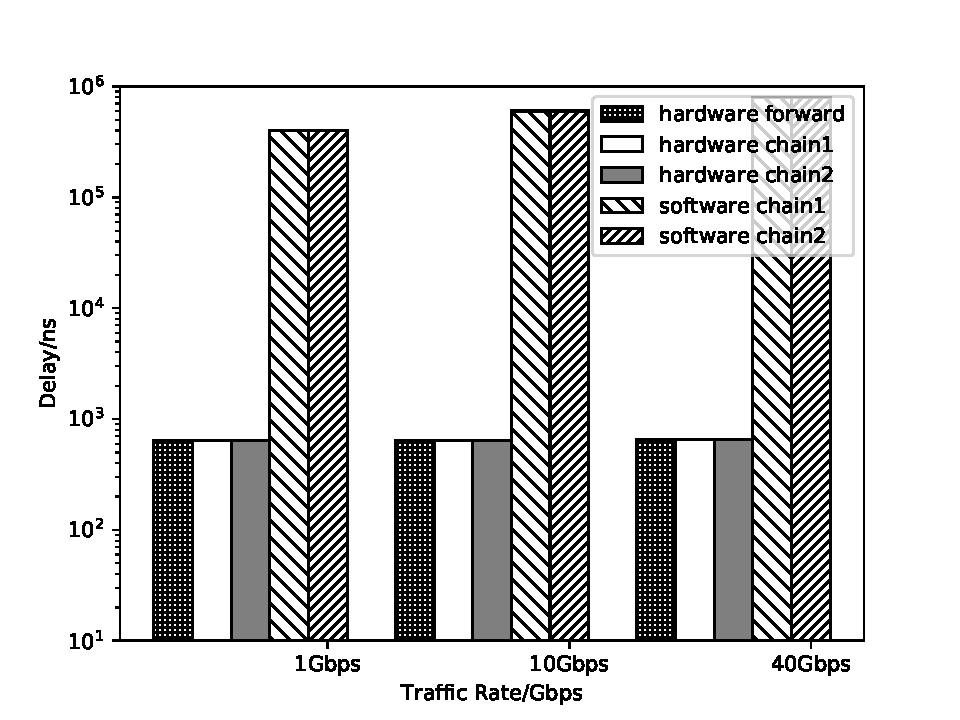
\includegraphics[width=0.45\linewidth]{src/single1.pdf}}  
\label{2a}
\subfloat[]{  
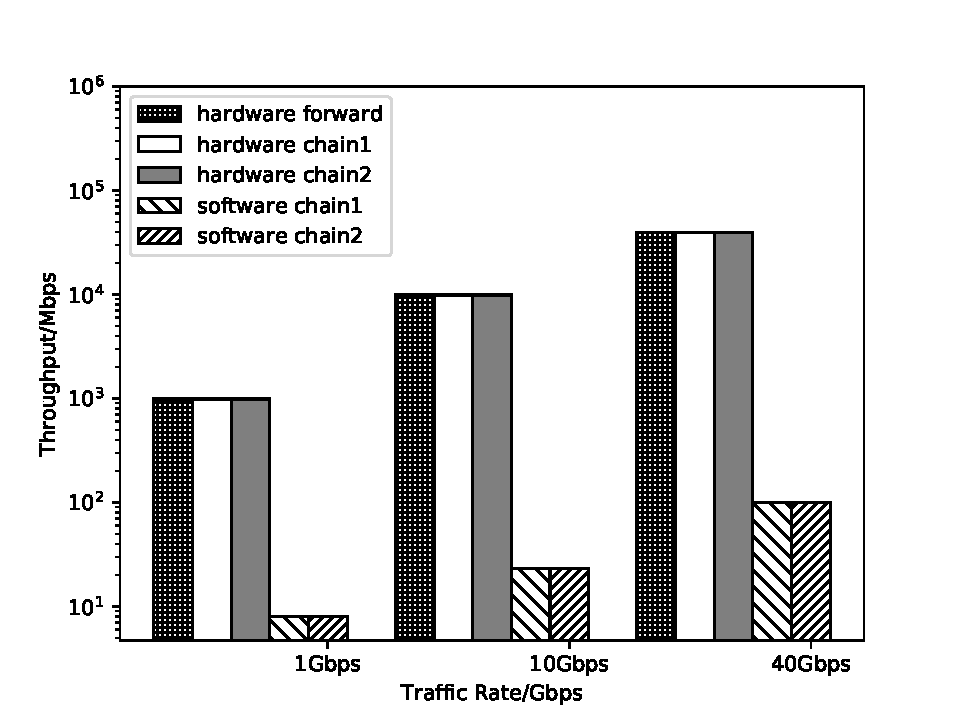
\includegraphics[width=0.45\linewidth]{src/single2.pdf}}  
\label{2b}\\
\caption{Latency and throughput result of hardware performance test}  
\label{hard}  
\end{figure} 

\subsection{Analytical Evaluation of Control Plane Algorithm}
\textbf{Experiment Setup}. We built the network topology with BMv2 switches on mininet with ONOS controller. We implemented the same HNFs as hardware experiment. The topology used is abilene in SDNlib with 12 nodes and 22 links, we also used the trace data set provided by SDNlib in the same topology, where traffic throughput of every node pairs are listed. We wrote the script to generate and receiver packets on different nodes, every flow in network is selected randomly from data set and is allocated with randomly selected service chain requirements. Flow completion time, throughput, link load and memory usage are informations collected to be evaluated. Implement the control plane(NF manage platform) based on ONOS controller with about 1000 LOC in JAVA. The control plane consists of modules: basic forward module, static algorithm module, dynamic algorithm module, NF rule translation module. We use Yen'algorithm[] to select k-shortest-path, and use the API provided by ONOS to collect metrics. In addition, we expands the ONOS framework to support the deployment of different P4 programs on different switches.

\textbf{Bechmark}.

\textbf{FCT and Throughput Performance}.

\textbf{Bandwidth Resources}.

\textbf{Flow Entry Resources}.


\section{Conclusion}
~\\


\section*{Acknowledgment}


\bibliographystyle{unsrt}  
\bibliography{StatefulPDP}
\cite{Bianchi2014}
\cite{Sun2017}
\cite{Li2016}
\cite{Pontarelli2019}
\cite{Dargahi2017}
\cite{Gember-Jacobson2015}
\cite{Sun2017}
\cite{sun2017hyper}
\cite{bosshart2014p4}
\cite{fujisawa2002sdpa}
\cite{sun2017hyper}
\cite{xu2016demystifying}
\cite{bifulco2018survey}
\cite{zheng2018p4visor}
\cite{zhang2019hypervdp}
\cite{hancock2016hyper4}

\end{document}
